\section{EXPERIMENTATION}
\subsection{Sensitivity Analysis}
\begin{frame}{EXPERIMENTATION}
    \framesubtitle{Sensitivity Analysis}
    \begin{itemize}
        \item Not enough data or rejected distributions $\rightarrow$ parameters or other distribution.
        \item Number of open modules.
    \end{itemize}
    \begin{figure}
        \centering
        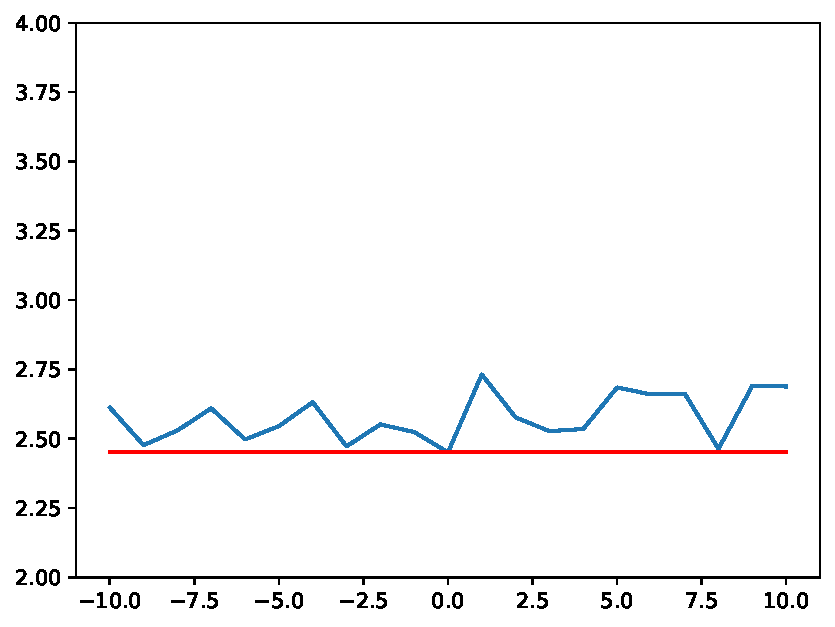
\includegraphics[scale=.5]{images/sensitivity.pdf}
        \caption{Sensitivity analysis $\pm$10\% in mean of assumed distributions.}
    \end{figure}
\end{frame}

\subsection{Optimization}
\begin{frame}{EXPERIMENTATION}
    \framesubtitle{Optimization}
    \begin{itemize}
        \item Minimize time in queue for each type of service.
        \item Best combination for priorities of Table \ref{tab:sets_priorities_opt}.
        \item Heuristic Approach $\rightarrow$ Local search $\rightarrow$ VNS.
    \end{itemize}
    \begin{multicols}{2}
    \begin{figure}
        \centering
        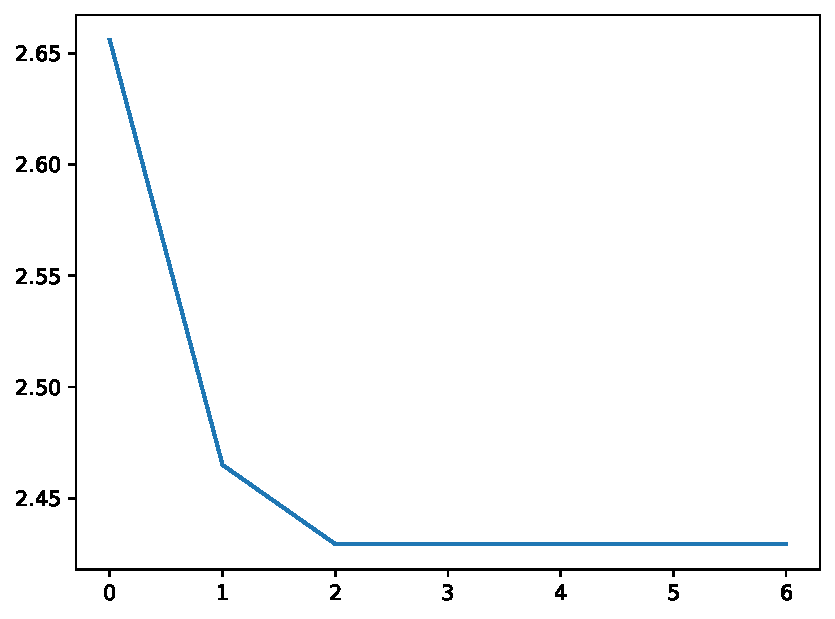
\includegraphics[scale=.4]{images/opti.pdf}
        \caption{Heuristic results}
    \end{figure}
    \columnbreak
    \begin{table}[H]
\centering
\begin{tabular}{cl}
\hline
\textbf{Set} & \textbf{Priority} \\ \hline
1            & {[}5, 4, 9{]}     \\
2            & {[}8, 10, 7, 3{]} \\
3            & {[}7, 3, 10, 8{]} \\
4            & {[}8, 10, 3, 7{]} \\
5            & {[}3, 7, 8, 10{]} \\
6            & {[}8, 3, 7, 10{]} \\ \hline
\end{tabular}
\caption{Sets and priorities.}
\label{tab:sets_priorities_opt}
\end{table}
    \end{multicols}
\end{frame}

